\section{Introduction and Goals}\label{sec:introduction-and-goals}
The goal of this document is to provide a comprehensive overview of the software architecture of the Typecode Registry.
It is intended to be used as a reference for developers, architects, and other stakeholders to understand
the system's architecture and to make informed decisions about the system's design and implementation.


\subsection{Requirements Overview}\label{subsec:requirements-overview}
\subsubsection{Motivation}\label{subsubsec:motivation}
In the realm of SAP Commerce, unique numbers, referred to as Typecodes, are internally allocated to its types.
Uniqueness of these numbers is a necessity within each individual project.
To address this, NETCONOMY introduced the
``Typecode Registry``.
This registry guarantees that every type within a project, as well as those within multi-project
extensions, is assigned a unique and non-reusable Typecode.
However, the current application has become outdated
and excessively complex, failing to meet the company's evolving requirements.
As a result, there is a need to redesign
the application in line with modern standards and needs.
The ultimate objective is to develop an application that offers
developers access to conflict-free Typecodes, thereby streamlining their daily operations.

\subsubsection{Contents}\label{subsubsec:contents}
The Typecode Registry is a system that provides a central repository for typecodes and their associated metadata.
A developer can use the system to reserve a typecode for a specific type (also called item), and the system will ensure
that the typecode is unique (following a specific rule set).
Typecodes can be created for extensions.
Those extensions can not only be associated with a project,
furthermore, they can be defined as global extensions, which are available for all projects.
There are some rules that need to be followed when creating a typecode.
The purpose of the system is to ease the process
of creating typecodes for a developer so that the developer does not need to worry about the uniqueness of the typecode
and can focus on the development of the project.

\newpage
The following goals have been established for the system:

\begin{table}[h]
\centering
\begin{tabular}{|l|p{0.8\textwidth}|}
\hline
\textbf{Priority} & \textbf{Description} \\ \hline
1 & The system shall consist of a web application and a backend connected to a database. \\ \hline
2 & The system shall provide a REST API allowing automated reservation and management of items. \\ \hline
3 & The system shall enable the creation of projects, which can contain multiple extensions allowing each extension to contain multiple items. \\ \hline
4 & Each item has a specific Scope (Hybris, Common, Project) which determines the generated type code number ranges. \\ \hline
5 & Projects, Extensions and Items can be created manually via the User Interface. \\ \hline
6 & The same typecode can be used in two different projects. \\ \hline
7 & Items can be imported via a ``ìtems.xml`` file. \\ \hline
8 & Internal system Typecodes can be imported via a ``reservedTypecodes.txt`` file by an administrator. \\ \hline
9 & The table listing the typecode shall offer the possibility to filter, sort and search for typecodes \\ \hline
10 & Users should be able to login by using their Microsoft Account. \\ \hline
\end{tabular}
\caption{Priorities}
\label{tab:priority-description}
\end{table}

\subsection{Requirements}\label{subsec:quality-objective}

\begin{figure}[H]
\hspace*{-0.5cm}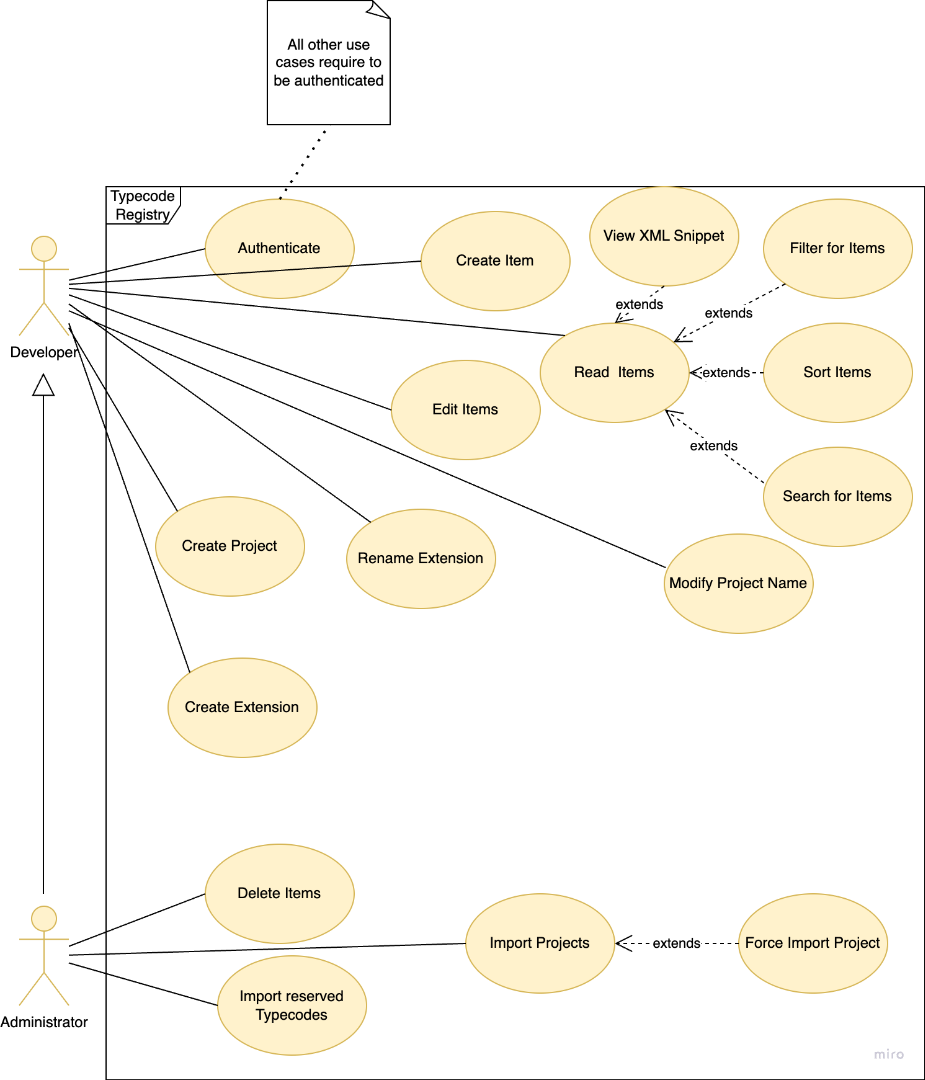
\includegraphics[scale=0.21]{images/introduction/use_cases}
\caption{Overview of the Use Cases}
\label{fig:use-cases}
\end{figure}

\begin{table}[H]
\centering
\begin{tabular}{|l|p{0.25\textwidth}|p{0.6\textwidth}|}
\hline
\textbf{ID} & \textbf{Requirement} & \textbf{Explanation} \\ \hline
F1 & Create an Item & Create an item over the UI.  \\ \hline
F2 & Edit an Item & An item which already exists in the system can be modified. \\ \hline
F3 & Read Items & Items which exist in the system shall be retrievable and displayed. \\ \hline
F3.1 & Display item's xml snippet & The xml snippet of the typecode shall be displayed.  \\ \hline
F3.2 & Filter for items & Displayed items can be filtered by name, typecode, table-name, extension ande scope.  \\ \hline
F3.3 & Sort items & Displayed items shall be sortable by name, extension, scope and project. \\ \hline
F3.4 & Search items & The list of typecodes displayed can be searched through via a search field. \\ \hline
F4 & Create a Project & Create a project over the UI. \\ \hline
F5 & Create an Extension & Create an extension over the UI. \\ \hline
F6 & Rename Extension & An extension which already exists in the system can be renamed. \\ \hline
F7 & Add item to extension & An item can be added to an extension. \\ \hline
F8 & Add extension to project & An extension can be added to a project. \\ \hline
F9 & Modify Project Name & A project which already exists in the system can be renamed. \\ \hline
F10 & Delete Items & An administrator has additionally the possibility to delete an item. \\ \hline
F11 & Import Reserved Typecodes & Internal system Typecodes can be imported via a ``reservedTypecodes.txt`` file by an administrator. \\ \hline
F12 & Import Projects & Projects can be imported via a XML file.
It shall be possible to force an import if the typecodes would overlapp with already existing Common or Hybris typecodes. \\ \hline
F13 & Remove Extensions from Project & An extension can be removed from a project by an administrator. \\ \hline
F14 & Login & Users should be able to login by using their Microsoft Account. \\ \hline
F15 & Logout & Users should be able to logout. \\ \hline
\end{tabular}
\caption{Requirements}
\label{tab:requirements}
\end{table}